\documentclass{article}

\usepackage{amsmath}
\usepackage[margin=1in]{geometry}
\usepackage{listings}
\usepackage{hyperref}
\usepackage{graphicx}
\usepackage{amssymb}
\usepackage{verbatim}
\usepackage{siunitx}
\usepackage{enumitem}
\usepackage{bbm}
\usepackage{bm}
\usepackage{caption}
\usepackage{algpseudocode}
\usepackage{algorithm}
\usepackage[square,sort,comma,numbers]{natbib}

\newcommand{\norm}[1]{\left\lVert#1\right\rVert}
\newcommand{\normtwo}[1]{\left\lVert#1\right\rVert_2}
\newcommand{\abs}[1]{\left\lvert#1\right\rvert}
\newcommand{\mat}[1]{\bm{{#1}}}
\renewcommand{\vec}[1]{\bm{{#1}}}
\newcommand{\lequiv}{\Leftrightarrow}
\newcommand{\bigO}[1]{\mathcal{O}\!\left(#1\right)}
\newcommand{\ceil}[1]{\left\lceil #1 \right\rceil}
\newcommand{\floor}[1]{\left\lfloor #1 \right\rfloor}
\newcommand{\sfrac}[2]{#1/#2}
\newcommand{\hquad}{\enskip}
\newcommand{\expected}[1]{\mathbb{E}\left[#1\right]}
\newcommand{\mspan}[1]{\text{span}\left( #1 \right)}
\newcommand{\prob}[1]{P\left(#1\right)}
\newcommand{\probt}[1]{P\left( \text{#1} \right)}
\newcommand{\condprob}[2]{P\left(#1 \:|\: #2\right)}
\newcommand{\condprobt}[2]{P\left(\text{#1} \:|\: \text{#2}\right)}
\newcommand{\bayes}[2]{\frac{\condprob{#2}{#1}\prob{#1}}{\prob{#2}}}
\newcommand{\bayesx}[3]{\frac{\condprob{#2}{#1}\prob{#1}}{\condprob{#2}{#1}\prob{#1} + \condprob{#2}{#3}\prob{#3}}}
\newcommand{\sech}{\text{sech}}
\newcommand*{\qed}{\hfill\ensuremath{\blacksquare}}%
\newcommand*{\vertbar}{\rule[-1ex]{0.5pt}{2.5ex}}
\newcommand*{\horzbar}{\rule[.5ex]{2.5ex}{0.5pt}}
\newcommand{\vect}[2]{\underline{{#1}}_{{#2}}}
\newcommand{\basisp}[1]{\underline{{p}}_{{#1}}}
\newcommand{\basisq}[1]{\underline{{q}}_{{#1}}}
\newcommand{\coeff}[1]{\underline{{a}}_{{#1}}}
\newcommand{\bestfit}{\underline{\bar{x}}}
\newcommand{\grad}{\nabla}
\newcommand{\laplace}{\Delta}


\begin{document}

\begin{figure}[h]
  \centering
  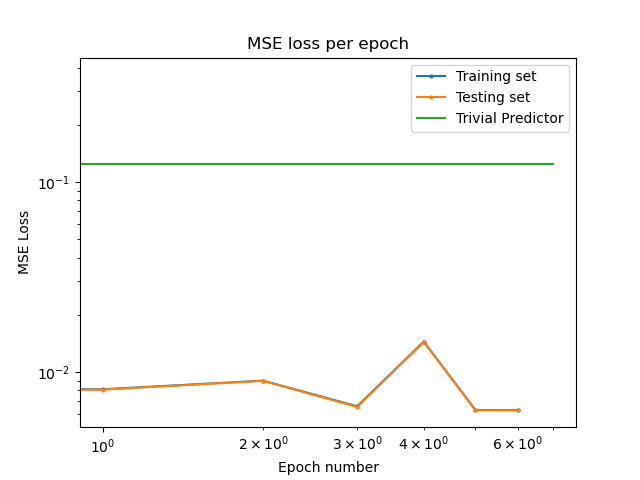
\includegraphics[scale=0.7]{figures/recircflow/conv_train_mse.png}
  \caption{(CNN) MSE loss per training iteration}
\end{figure}

\begin{figure}[h]
  \centering
  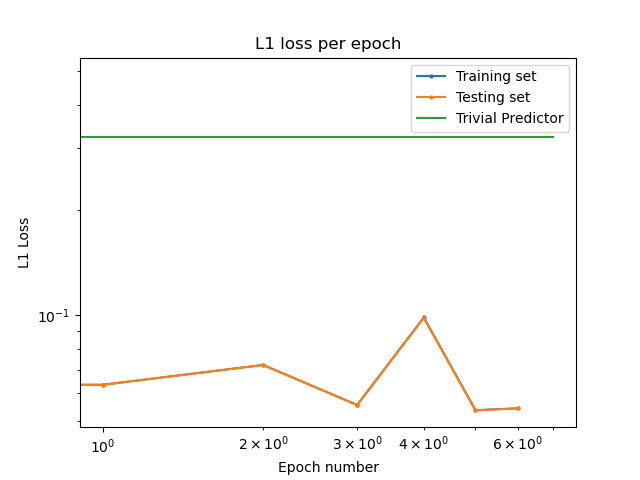
\includegraphics[scale=0.7]{figures/recircflow/conv_train_l1.png}
  \caption{(CNN) L1 loss per training iteration}
\end{figure}

\begin{figure}[h]
  \centering
  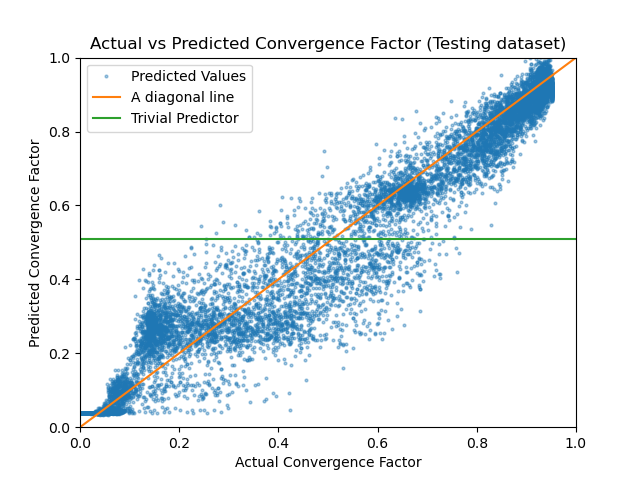
\includegraphics[scale=0.7]{figures/recircflow/conv_test_pred.png}
  \caption{(CNN) Predicted vs Actual Convergence Factor (Testing Dataset)}
  \label{fig:test}
\end{figure}

\begin{figure}[h]
  \centering
  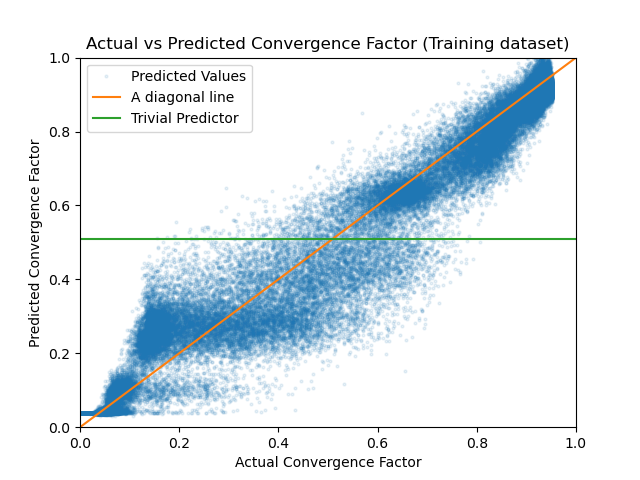
\includegraphics[scale=0.7]{figures/recircflow/conv_train_pred.png}
  \caption{(CNN) Predicted vs Actual Convergence Factor (Training Dataset)}
  \label{fig:train}
\end{figure}


\begin{figure}[h]
  \centering
  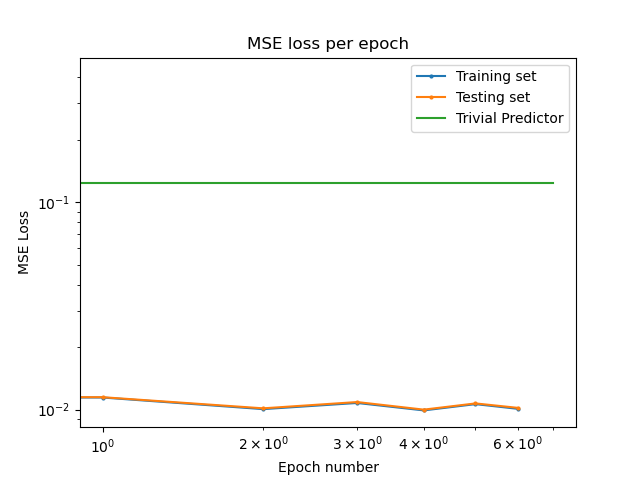
\includegraphics[scale=0.7]{figures/recircflow/gnn_train_mse.png}
  \caption{(GNN) MSE loss per training iteration}
\end{figure}

\begin{figure}[h]
  \centering
  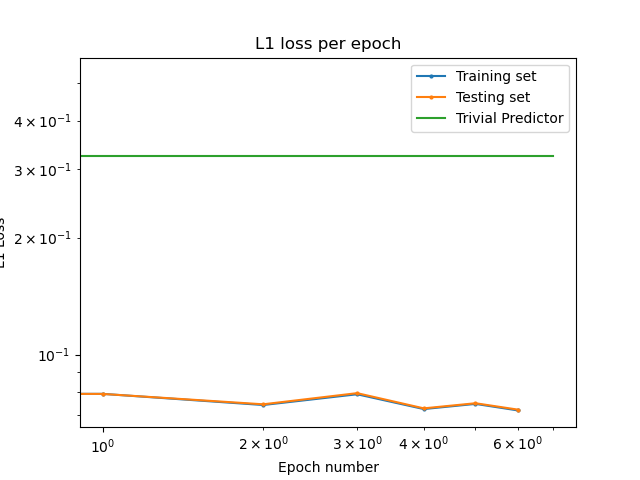
\includegraphics[scale=0.7]{figures/recircflow/gnn_train_l1.png}
  \caption{(GNN) L1 loss per training iteration}
\end{figure}

\begin{figure}[h]
  \centering
  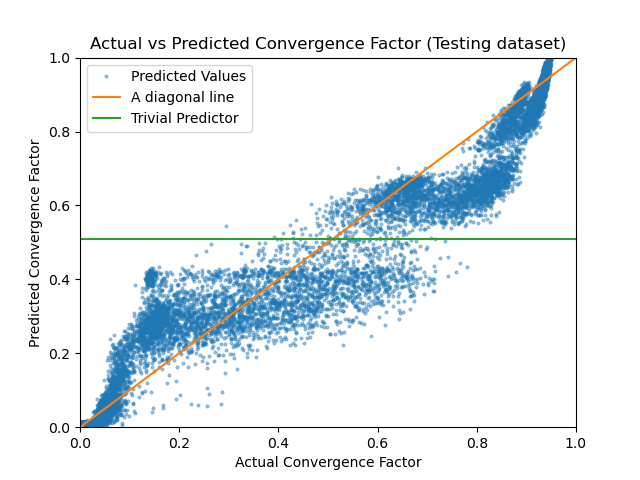
\includegraphics[scale=0.7]{figures/recircflow/gnn_test_pred.png}
  \caption{(GNN) Predicted vs Actual Convergence Factor (Testing Dataset)}
  \label{fig:test}
\end{figure}

\begin{figure}[h]
  \centering
  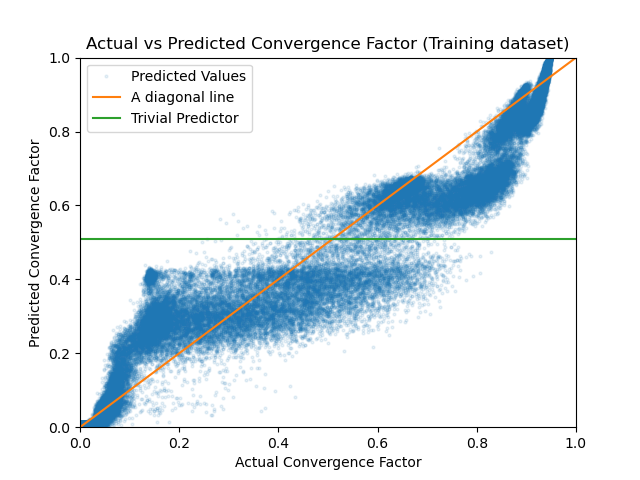
\includegraphics[scale=0.7]{figures/recircflow/gnn_train_pred.png}
  \caption{(GNN) Predicted vs Actual Convergence Factor (Training Dataset)}
  \label{fig:train}
\end{figure}

\begin{figure}[h]
  \centering
  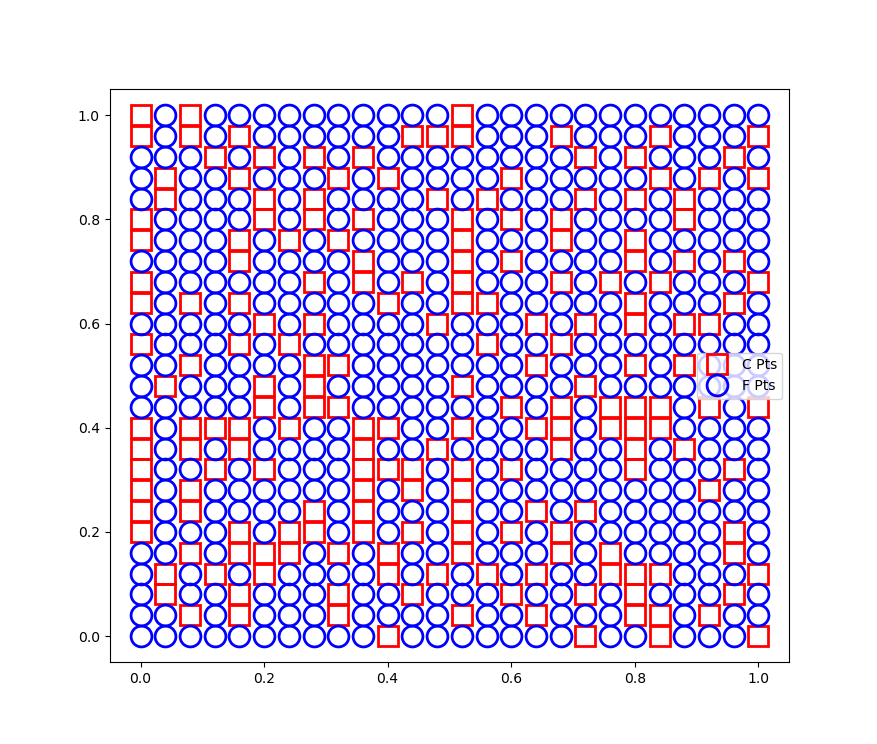
\includegraphics[scale=0.5]{figures/recircflow/gnn_grid_worst.png}
  \caption{(GNN) Worst predicted grid.  Actual convergence factor $0.7252$, predicted $0.3256$.}
  \label{fig:train}
\end{figure}

\end{document}
